\documentclass{article}
\usepackage{amsmath,amsfonts,amsthm,amssymb}
\usepackage{fullpage,fancyhdr}
\usepackage[pdftex]{graphicx}
\usepackage[usenames,dvipsnames]{color}
\usepackage{listings}
\usepackage{courier}
\usepackage{ifthen}
\usepackage{setspace}
\usepackage{lastpage}
\usepackage{extramarks}
\usepackage{chngpage}
\usepackage{soul}
\usepackage{graphicx,float,wrapfig}
\usepackage{epstopdf}
\usepackage{geometry}
\usepackage{pdfcolmk}
\usepackage{hyperref}
\DeclareGraphicsRule{.tif}{png}{.png}{`convert #1 `dirname #1`/`basename #1 .tif`.png}

\definecolor{lightgray}{gray}{0.5}
\definecolor{darkgray}{gray}{0.3}
\definecolor{MyDarkGreen}{rgb}{0.0,0.4,0.0}

\topmargin=-0.46in      %
\evensidemargin=0in     %
\oddsidemargin=0in      %
\textwidth=6.6in        %
\textheight=9.0in       %
\headsep=0.26in         %

\pagestyle{fancyplain}

% For faster processing, load Matlab syntax for listings
\lstloadlanguages{Matlab}%
\lstset{language=Matlab,
        frame=single,
        basicstyle=\ttfamily,
        keywordstyle=[1]\color{Blue}\bf,
        keywordstyle=[2]\color{Purple},
        keywordstyle=[3]\color{Blue}\underbar,
        identifierstyle=,
        commentstyle=\usefont{T1}{pcr}{m}{sl}\color{MyDarkGreen}\small,
        stringstyle=\color{Purple},
        showstringspaces=false,
        tabsize=5,
        % Put standard MATLAB functions not included in the default
        % language here
        morekeywords={xlim,ylim,var,alpha,factorial,poissrnd,normpdf,normcdf},
        % Put MATLAB function parameters here
        morekeywords=[2]{on, off, interp},
        % Put user defined functions here
        morekeywords=[3]{FindESS},
        morecomment=[l][\color{Blue}]{...},
        numbers=left,
        firstnumber=1,
        numberstyle=\tiny\color{Blue},
        stepnumber=5
        }

 
\fancyhf{}
 
\lhead{\fancyplain{}{Michael Carroll}}
\chead{\fancyplain{}{ELEC6410 - DSP}}
\rhead{\fancyplain{}{\today}}
\rfoot{\fancyplain{}{\thepage\ of \pageref{LastPage}}}

\sloppy
\setlength{\parindent}{0pt}

% Alter some LaTeX defaults for better treatment of figures:
% See p.105 of "TeX Unbound" for suggested values.
% See pp. 199-200 of Lamport's "LaTeX" book for details.
%   General parameters, for ALL pages:
\renewcommand{\topfraction}{0.9}	% max fraction of floats at top
\renewcommand{\bottomfraction}{0.8}	% max fraction of floats at bottom
%   Parameters for TEXT pages (not float pages):
\setcounter{topnumber}{2}
\setcounter{bottomnumber}{2}
\setcounter{totalnumber}{4}     % 2 may work better
\setcounter{dbltopnumber}{2}    % for 2-column pages
\renewcommand{\dbltopfraction}{0.9}	% fit big float above 2-col. text
\renewcommand{\textfraction}{0.07}	% allow minimal text w. figs
%   Parameters for FLOAT pages (not text pages):
\renewcommand{\floatpagefraction}{0.7}	% require fuller float pages
% N.B.: floatpagefraction MUST be less than topfraction !!
\renewcommand{\dblfloatpagefraction}{0.7}	% require fuller float pages
% remember to use [htp] or [htpb] for placement

\linespread{1.3}

\title{ELEC6410 Project 7\\
 {\large \begin{par}
Answers to Digital Signal Processing Project \#7
\end{par}
}}
\author{Michael J. Carroll}

\begin{document}
\maketitle
           
\section*{Exercise 1}
\begin{par}
For Exercise 1, I evaluated designing an FIR filter for five of the window types included in MATLAB.  These five windows were the rectangular, triangular, Hanning, Hamming, and Blackman windows.\\
\end{par}

\begin{par}
Each of the four windows demonstrate a tradeoff in the magnitude response.  The filter designed with the rectangular window in Figure 1 has a sharper transition band, but less attenuation and more stopband ripple.  The triangular window in Figure 2 has an equally sharp transition band, but significantly less stopband ripple.\\
\\
The Hanning, Hamming, and Blackman windowed filters (in Figures 3, 4, and 5, respectively) have much higher attenuation in the stopband, but the transition band is much wider, which would not make these filters ideal for picking off two frequencies close to each other.
\end{par}
\begin{figure}[htbp]
\centering
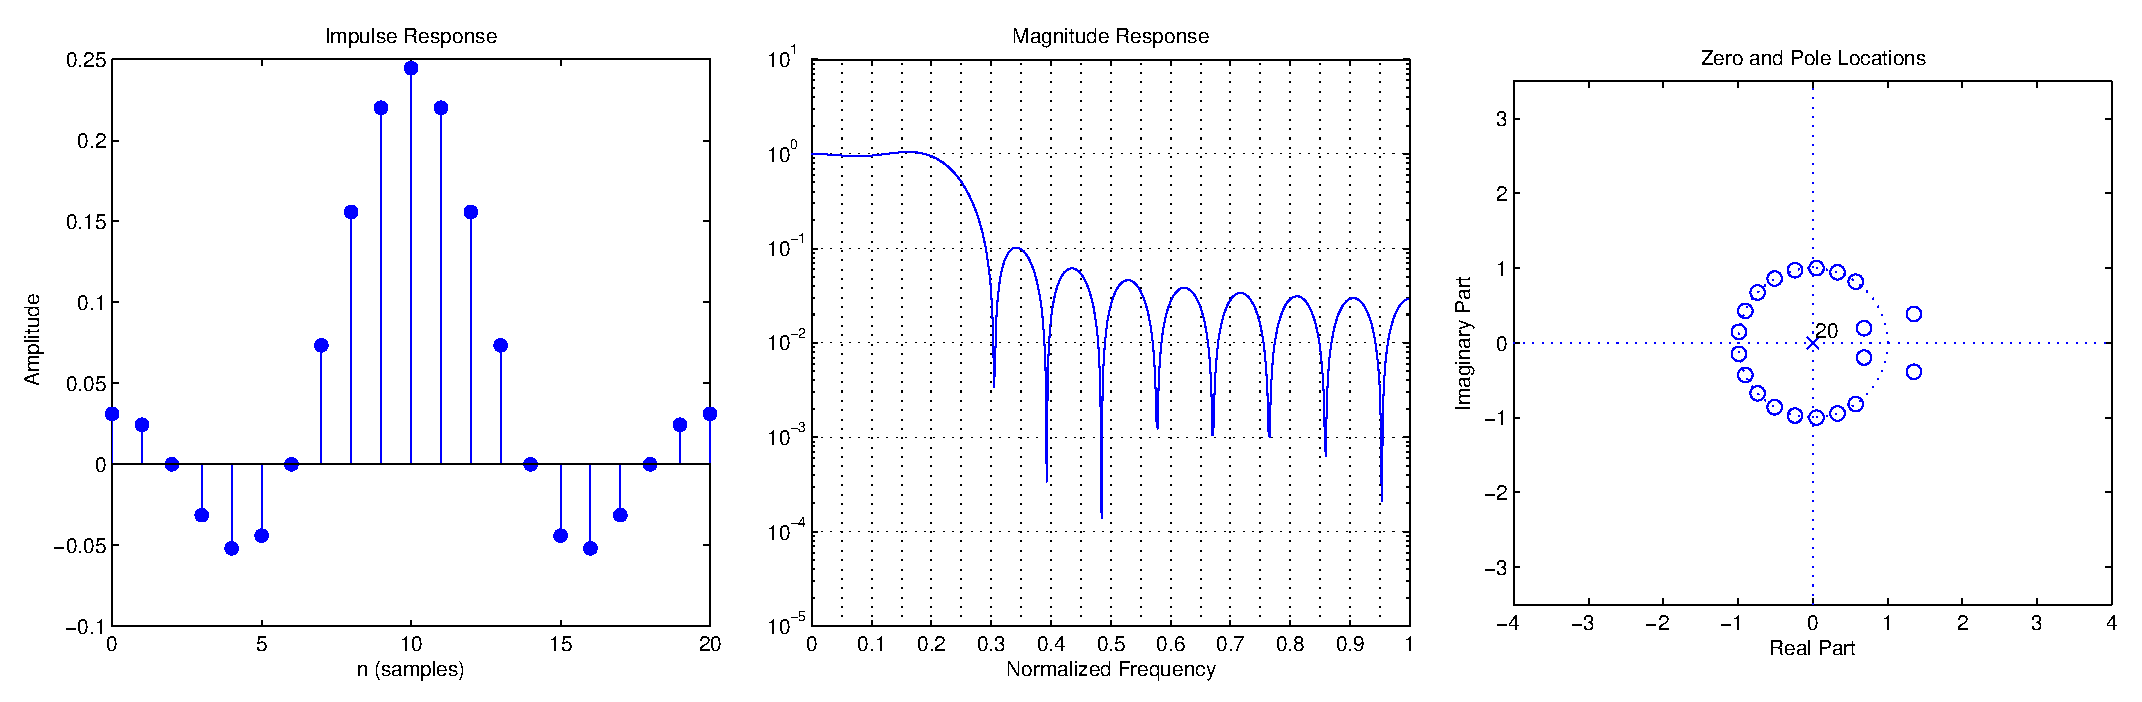
\includegraphics[width=6in]{project7_01.eps}
\caption{Response plots of FIR filter designed with rectangular window}
\label{fig:figure1}
\end{figure}

\begin{figure}[htbp]
\centering
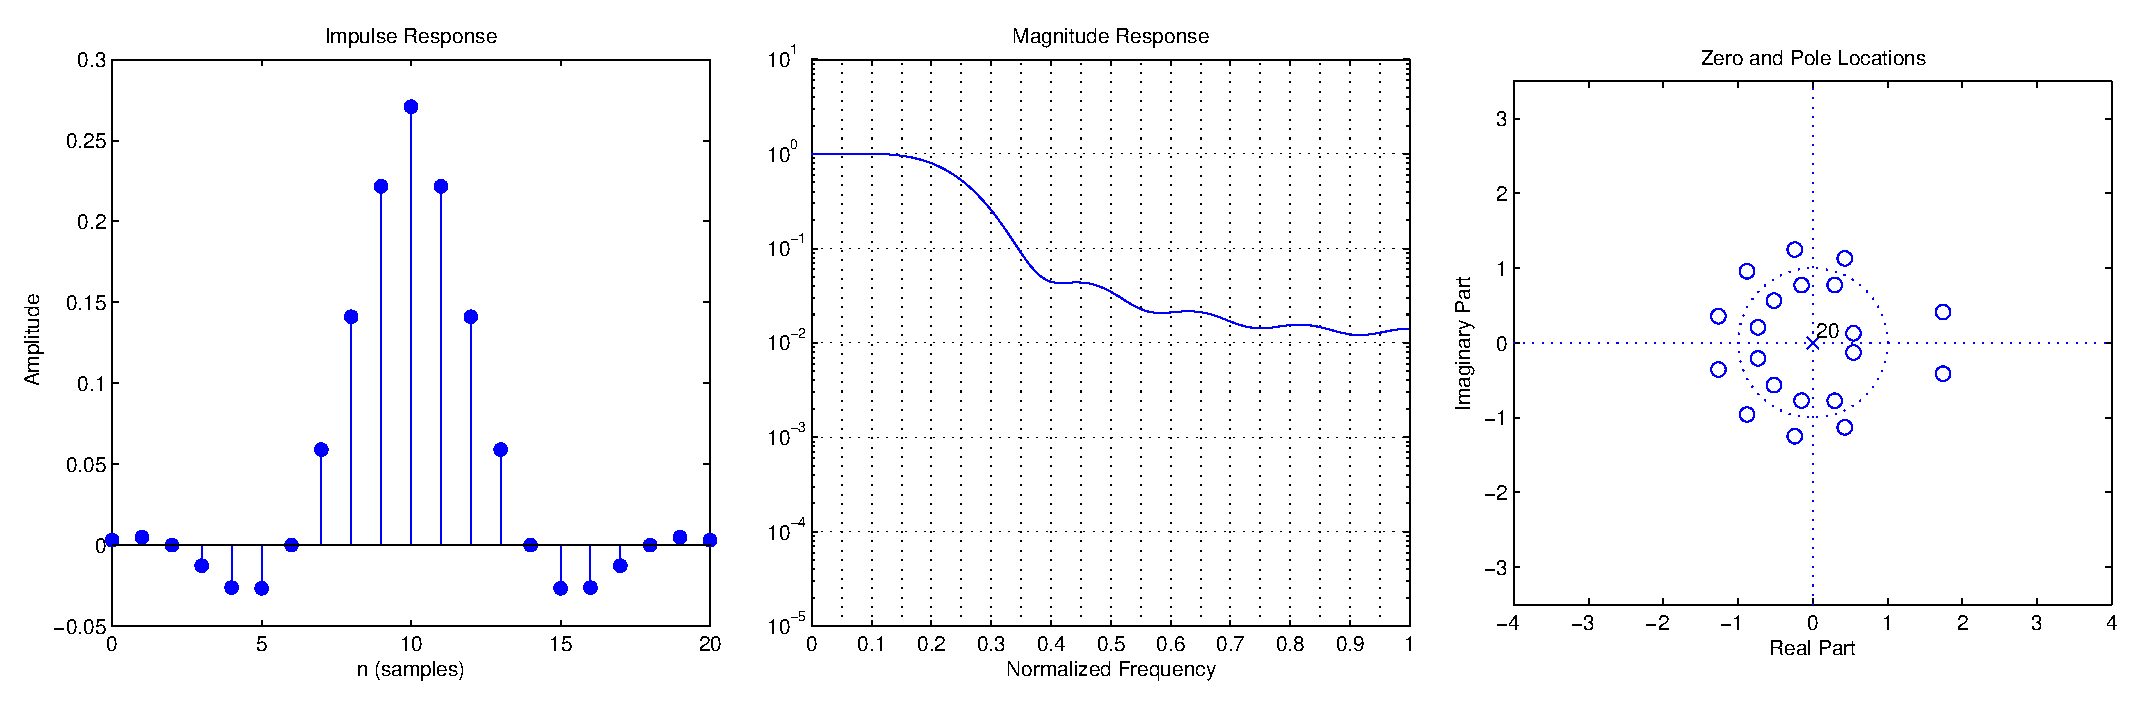
\includegraphics[width=6in]{project7_02.eps}
\caption{Response plots of FIR filter designed with triangular window}
\label{fig:figure2}
\end{figure}

\begin{figure}[htbp]
\centering
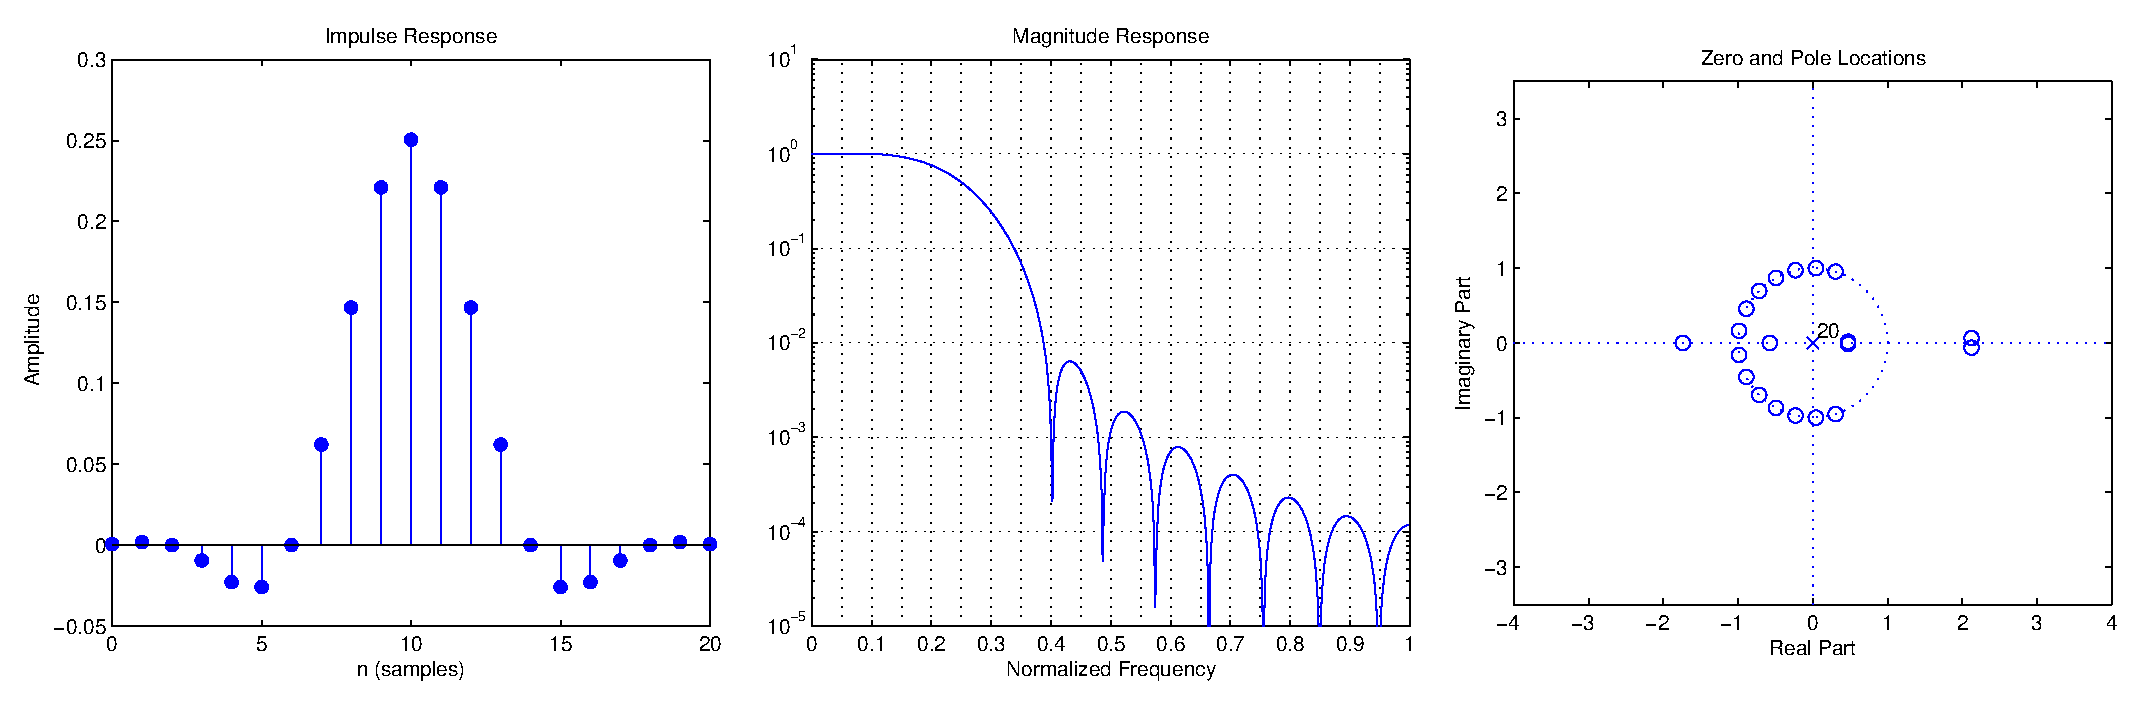
\includegraphics[width=6in]{project7_03.eps}
\caption{Response plots of FIR filter with Hanning window}
\label{fig:figure3}
\end{figure}

\begin{figure}[htbp]
\centering
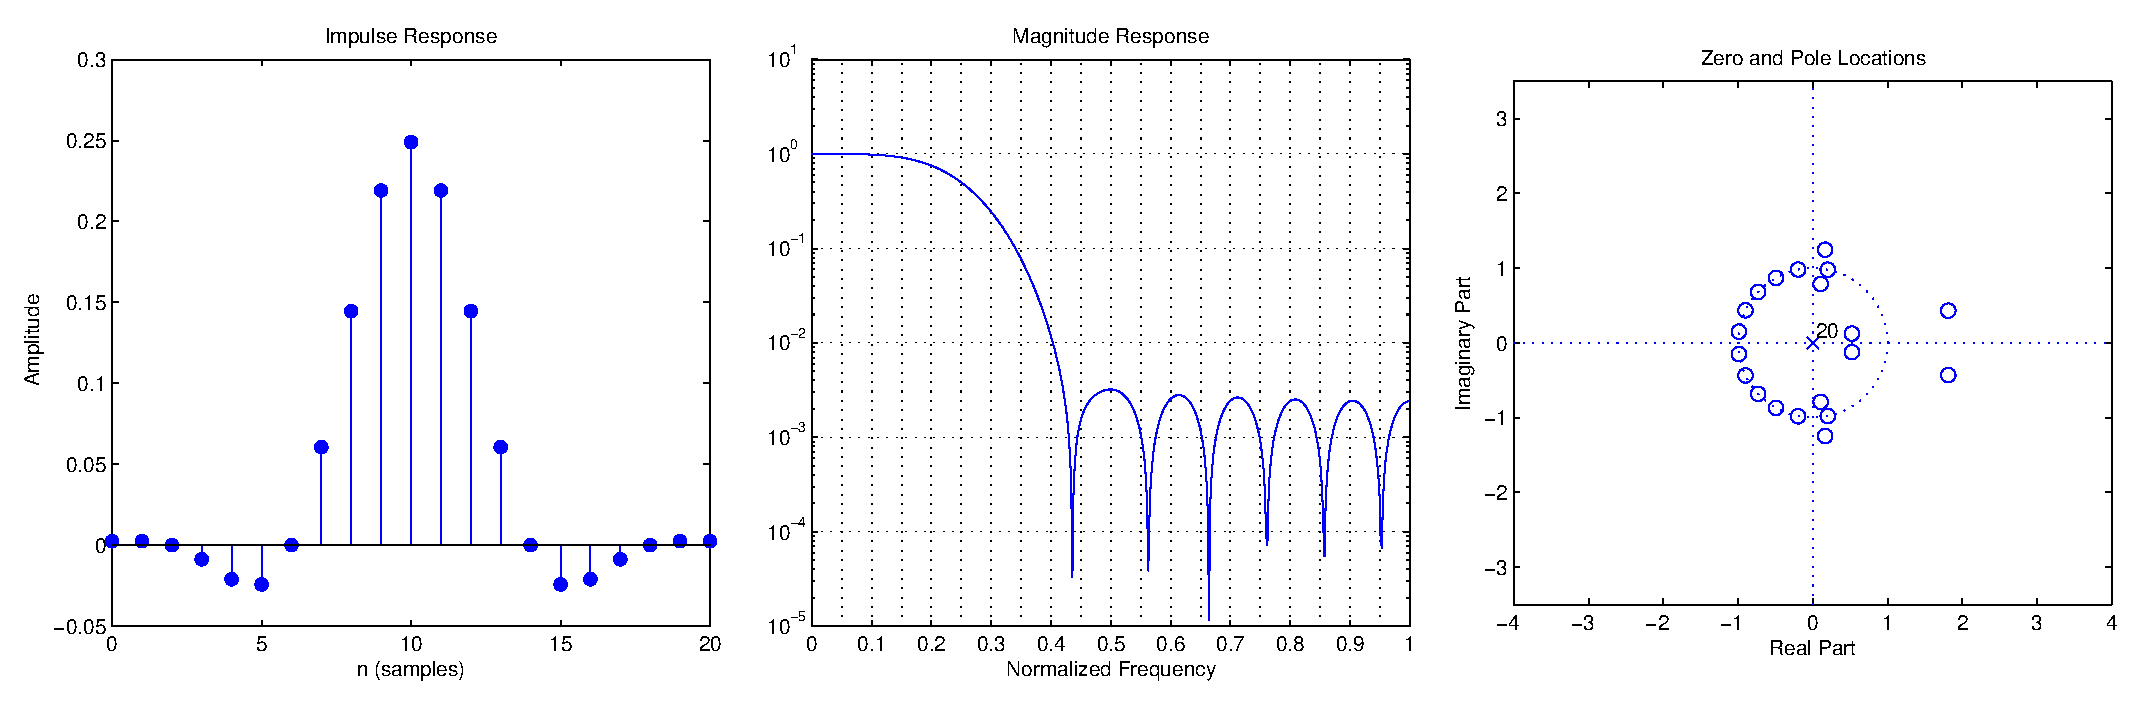
\includegraphics[width=6in]{project7_04.eps}
\caption{Response plots of FIR filter designed with Hamming window}
\label{fig:figure4}
\end{figure}

\begin{figure}[htbp]
\centering
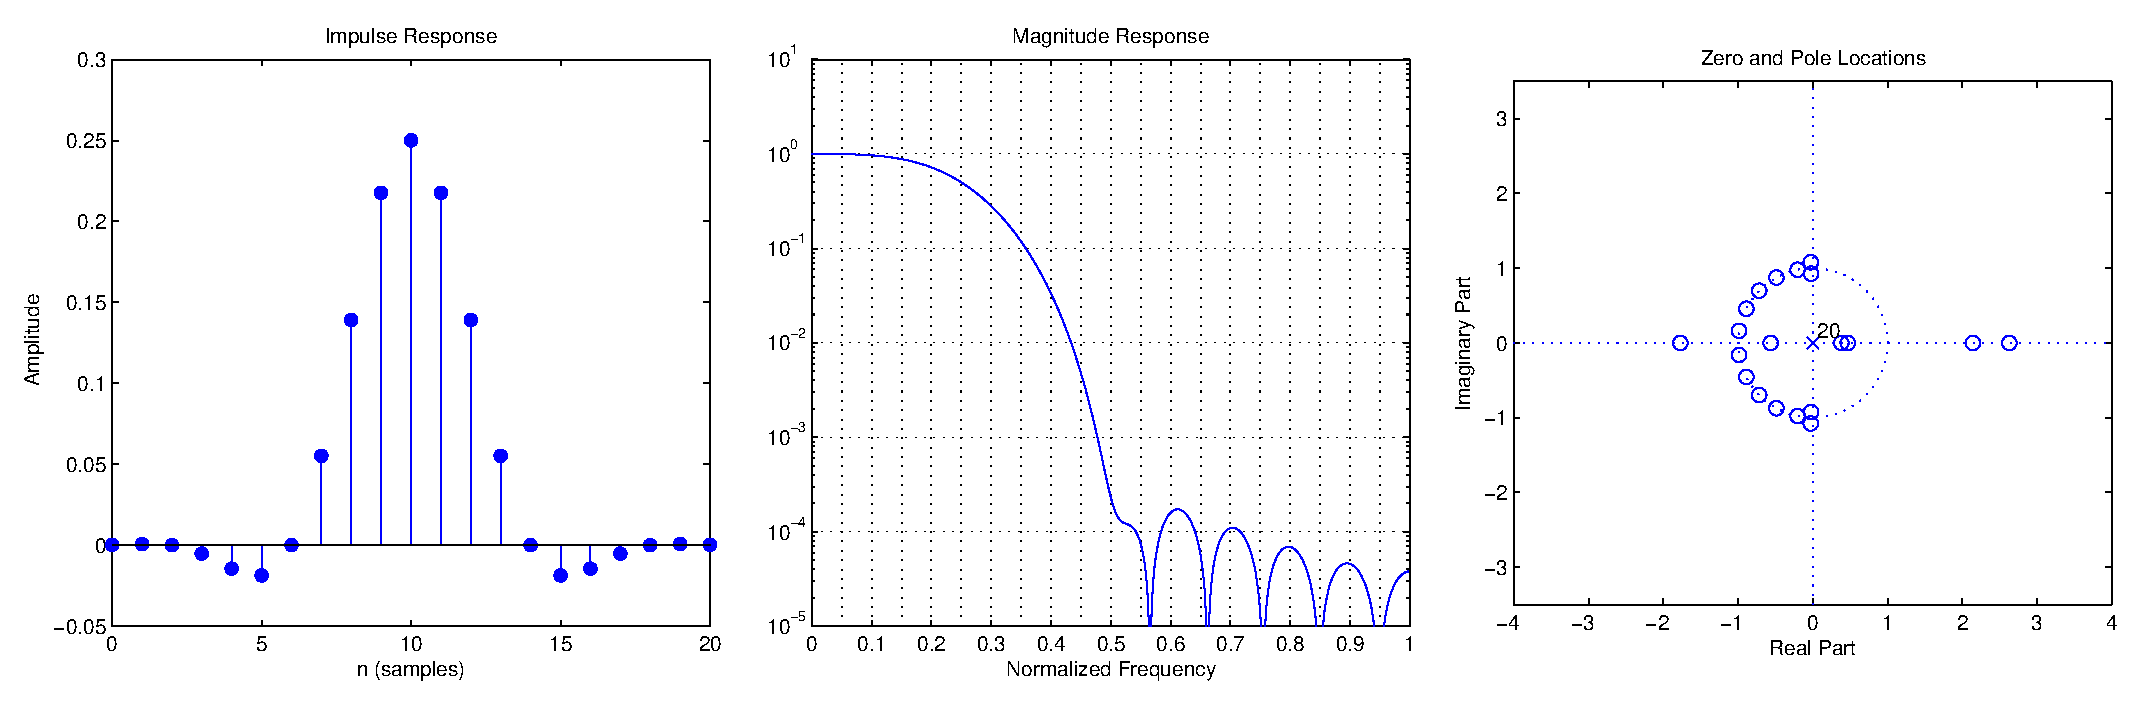
\includegraphics[width=6in]{project7_05.eps}
\caption{Response plots of FIR filter designed with Blackman window}
\label{fig:figure5}
\end{figure}

\newpage
\section*{Exercise 2}
\begin{par}
For Exercise 2, I designed an FIR lowpass filter using a Kaiser window with $\beta = 4, 6, 9$.  As the $\beta$ value increases in the Kaiser window, the magnitude characteristics of the filter change.  A higher $\beta$ yields a higher attenuation in the stopband of the filter, and reduces some of the ripple in the stopband.  Also, as a tradeoff, the transition band becomes much wider.  If a sharper transition band is required for a particular design, then a lower $\beta$ value would give better results.
\end{par}

\begin{figure}[htbp]
\centering
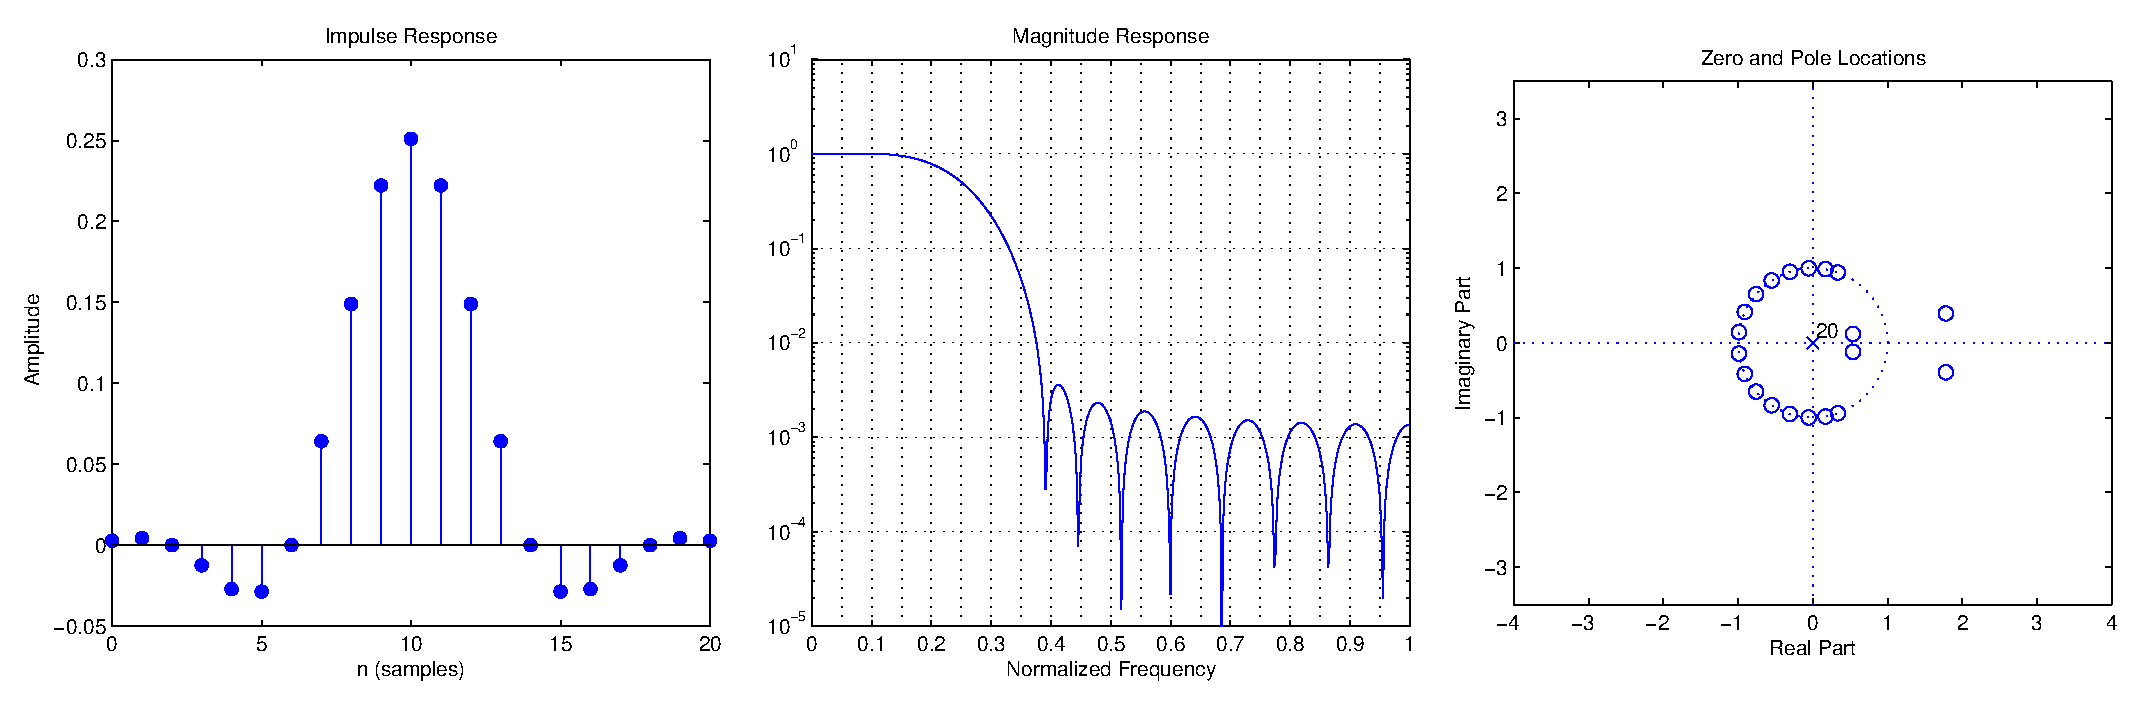
\includegraphics[width=6in]{project7_06.eps}
\caption{Response plots of FIR filter designed with Kaiser window, $\beta = 4$}
\label{fig:figure6}
\end{figure}

\begin{figure}[htbp]
\centering
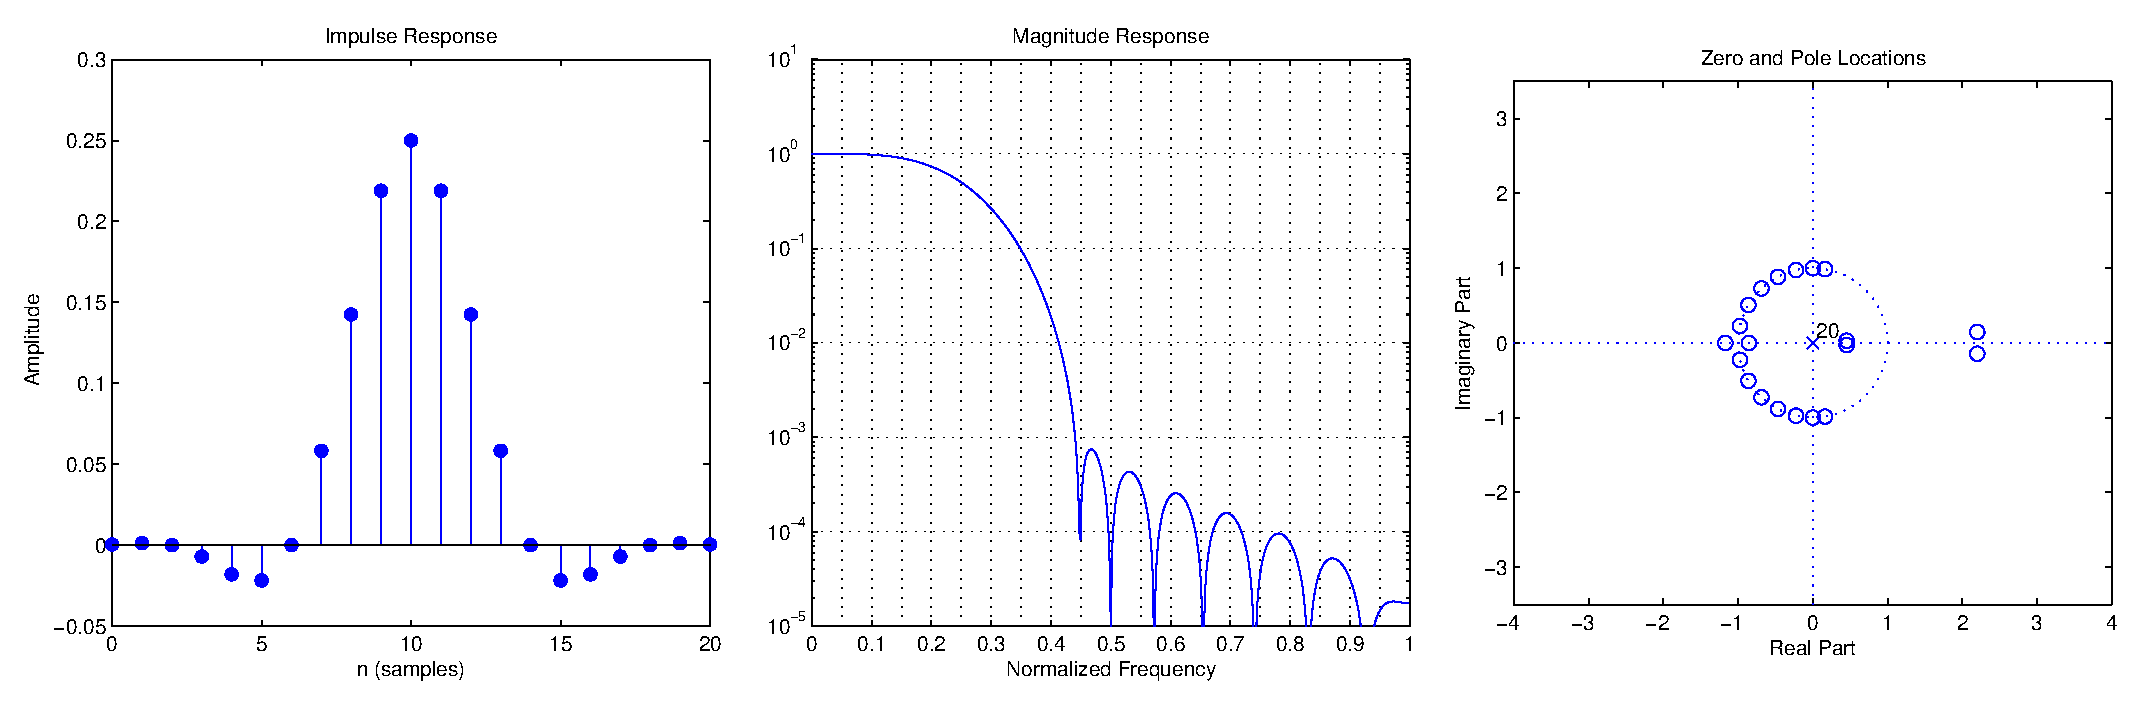
\includegraphics[width=6in]{project7_07.eps}
\caption{Response plots of FIR filter designed with Kaiser window, $\beta = 6$}
\label{fig:figure7}
\end{figure}

\begin{figure}[htbp]
\centering
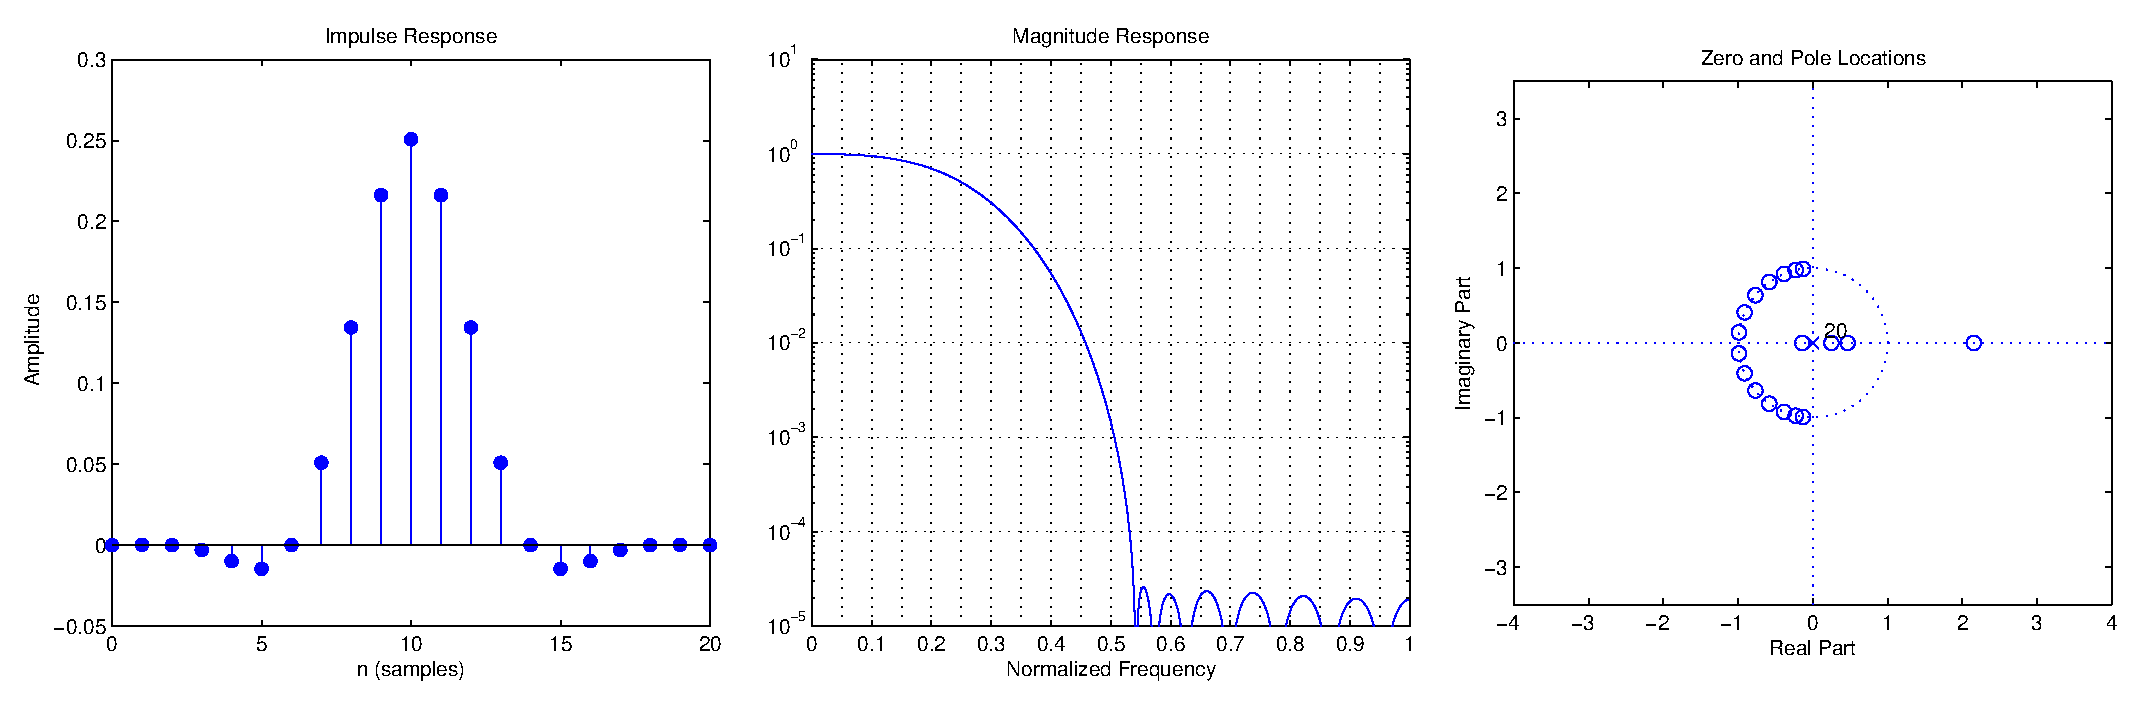
\includegraphics[width=6in]{project7_08.eps}
\caption{Response plots of FIR filter designed with Kaiser window, $\beta = 9$}
\label{fig:figure8}
\end{figure}

\newpage
\section*{Exercise 3}
\begin{par}
For Exercise 3, I designed an FIR lowpass filter using the frequency sampling method.  My code to do the frequency sampling is included below.  The results of the filter design are in Figure 9.  The frequency sampling method yields a good filter, but it has more passband ripple than some of the previous designs.  The stopband ripple is comparable to the Hanning, Hamming, and Blackman windows.
\end{par}

\begin{lstlisting}
N = 21; Wn = 0.25*pi;
freq = -pi:2*pi/(N-1):pi;
samp = circshift(abs(freq) < Wn,[0 ceil(N/2)]);
samp_B = circshift(ifft(samp),[0 ceil(N/2)]);
\end{lstlisting}

\begin{figure}[htbp]
\centering
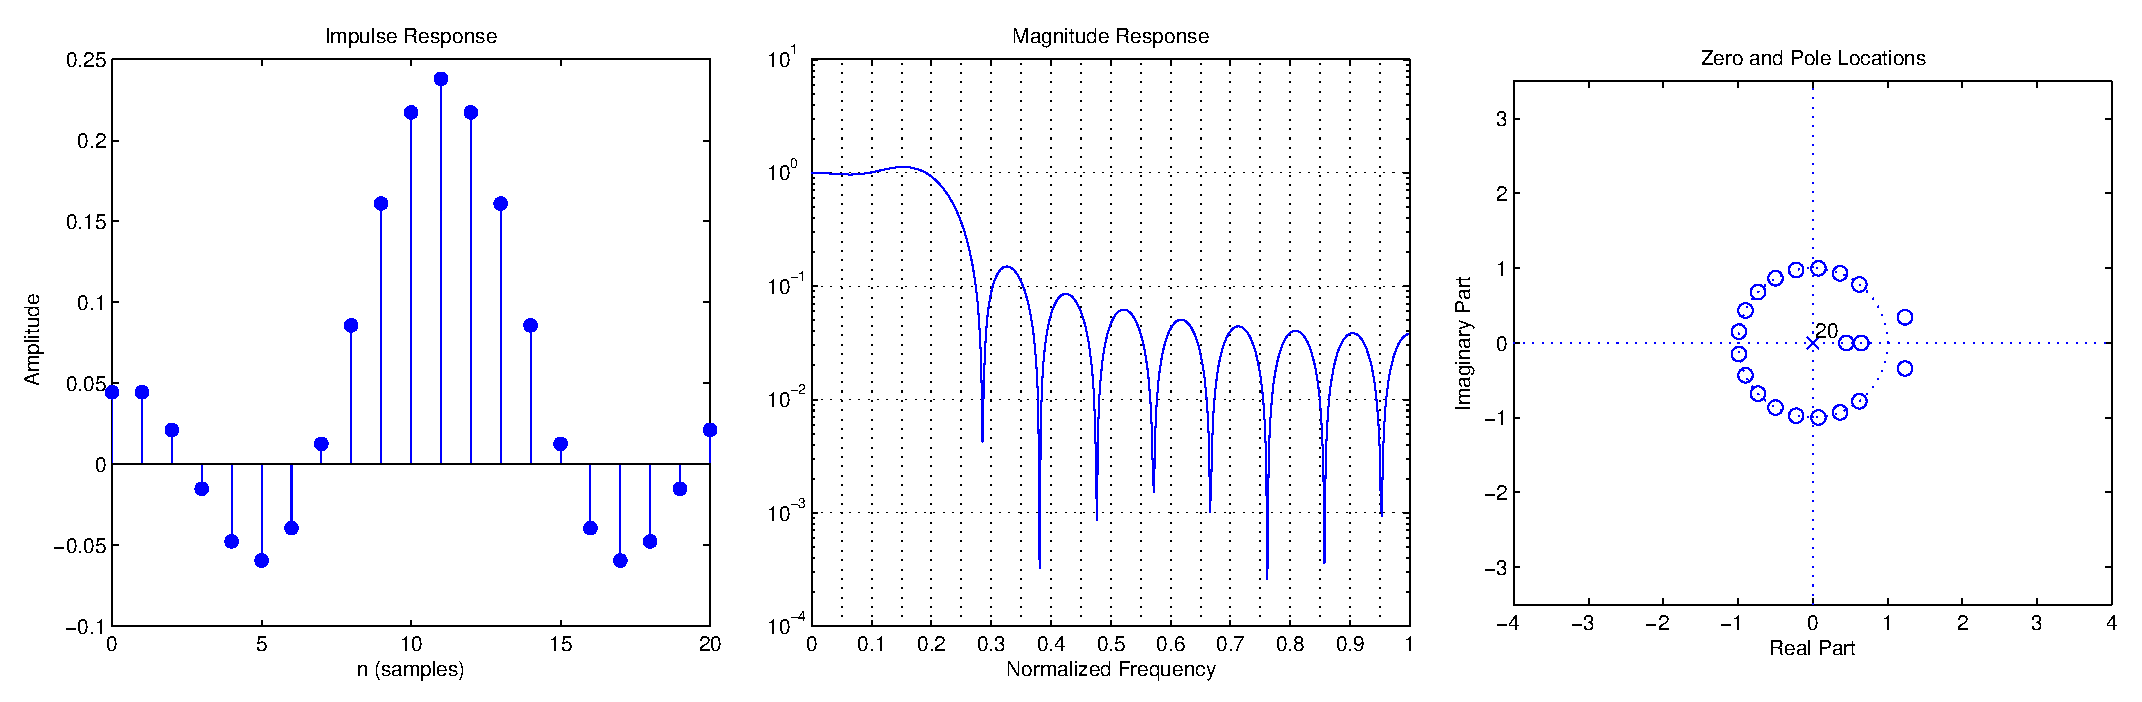
\includegraphics[width=6in]{project7_09.eps}
\caption{Response plots of FIR filter designed with frequency sampling method}
\label{fig:figure9}
\end{figure}

\newpage
\section*{Exercise 4}
\begin{par}
For Exercise 4, I designed an FIR lowpass filter using the Parks-McClellan algorithm.  The FIR filter response, included in Figure 10,  has a higher passband ripple than some of the other designs, but gives an all-around good filter.  The stopband ripple is comparable to some of the previous designs.
\end{par}

\begin{figure}[htbp]
\centering
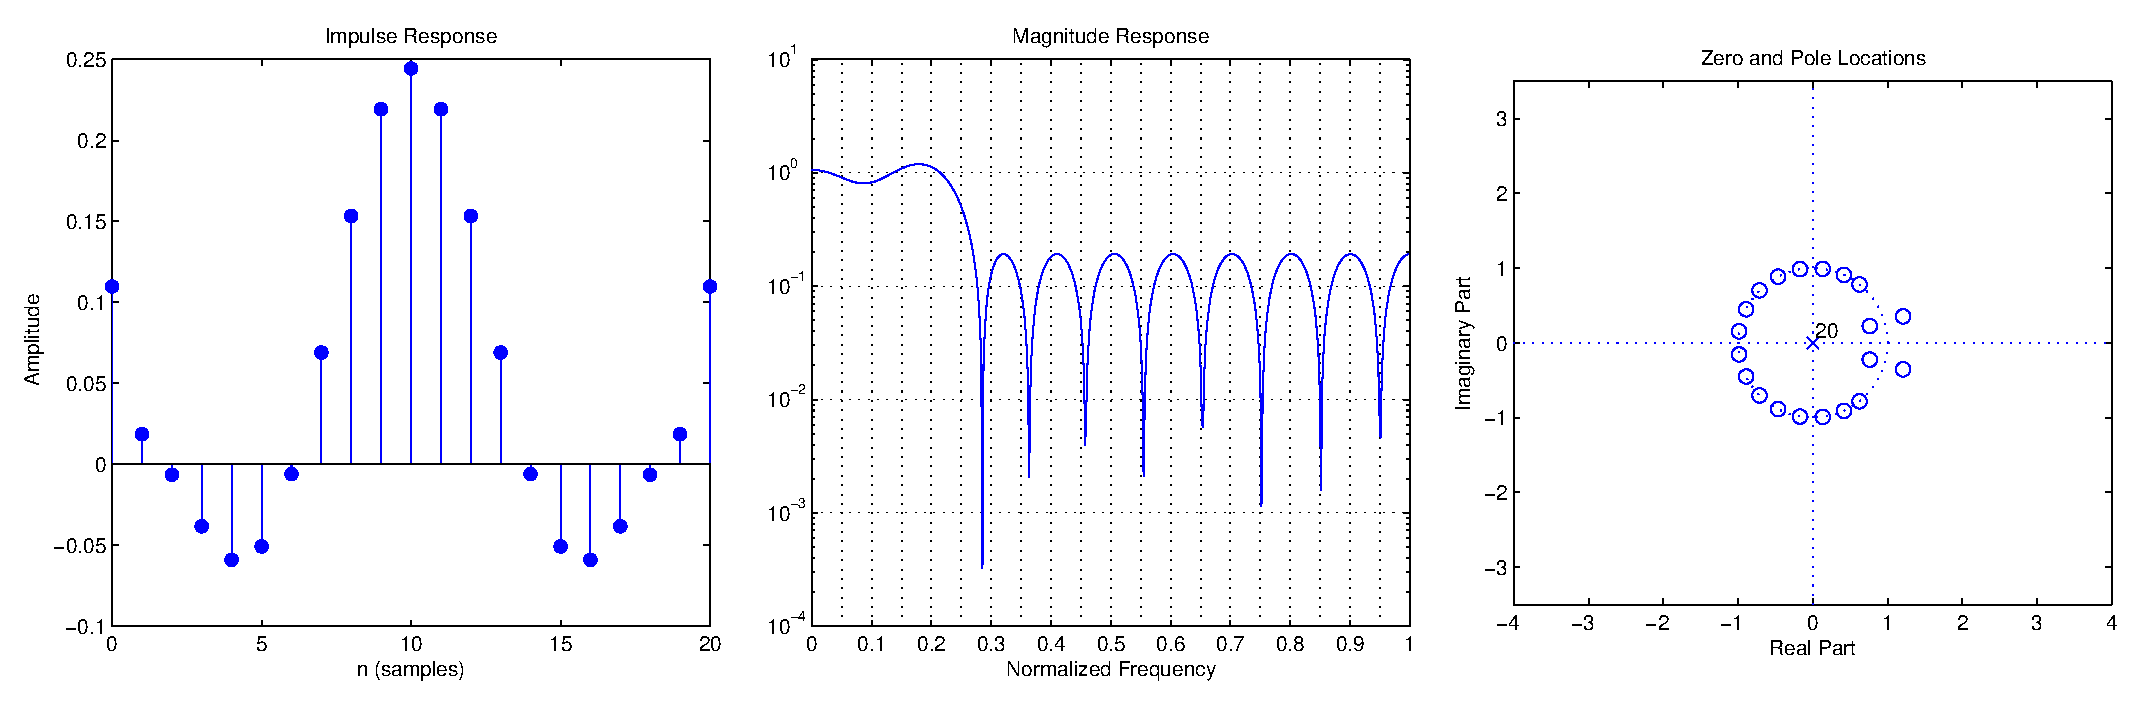
\includegraphics[width=6in]{project7_10.eps}
\caption{Response plots of FIR filter designed with Parks-McClellan}
\label{fig:figure10}
\end{figure}

\section*{Exercise 5}
\begin{par}
For Exercise 5, I designed an elliptical IIR lowpass filter to compare to the FIR filters that I designed.  The maximum attenuation achievable in the passband with an 11th order filter is 86dB.  The IIR filter of lower order, but equal computational complexity, has a much sharper transition band, but a less uniform stopband ripple.  The passband ripple is also much higher than the designs using the Kaiser window.  For most applications, an FIR filter would probably give equivalent results in less computation power.
\end{par}

\begin{figure}[htbp]
\centering
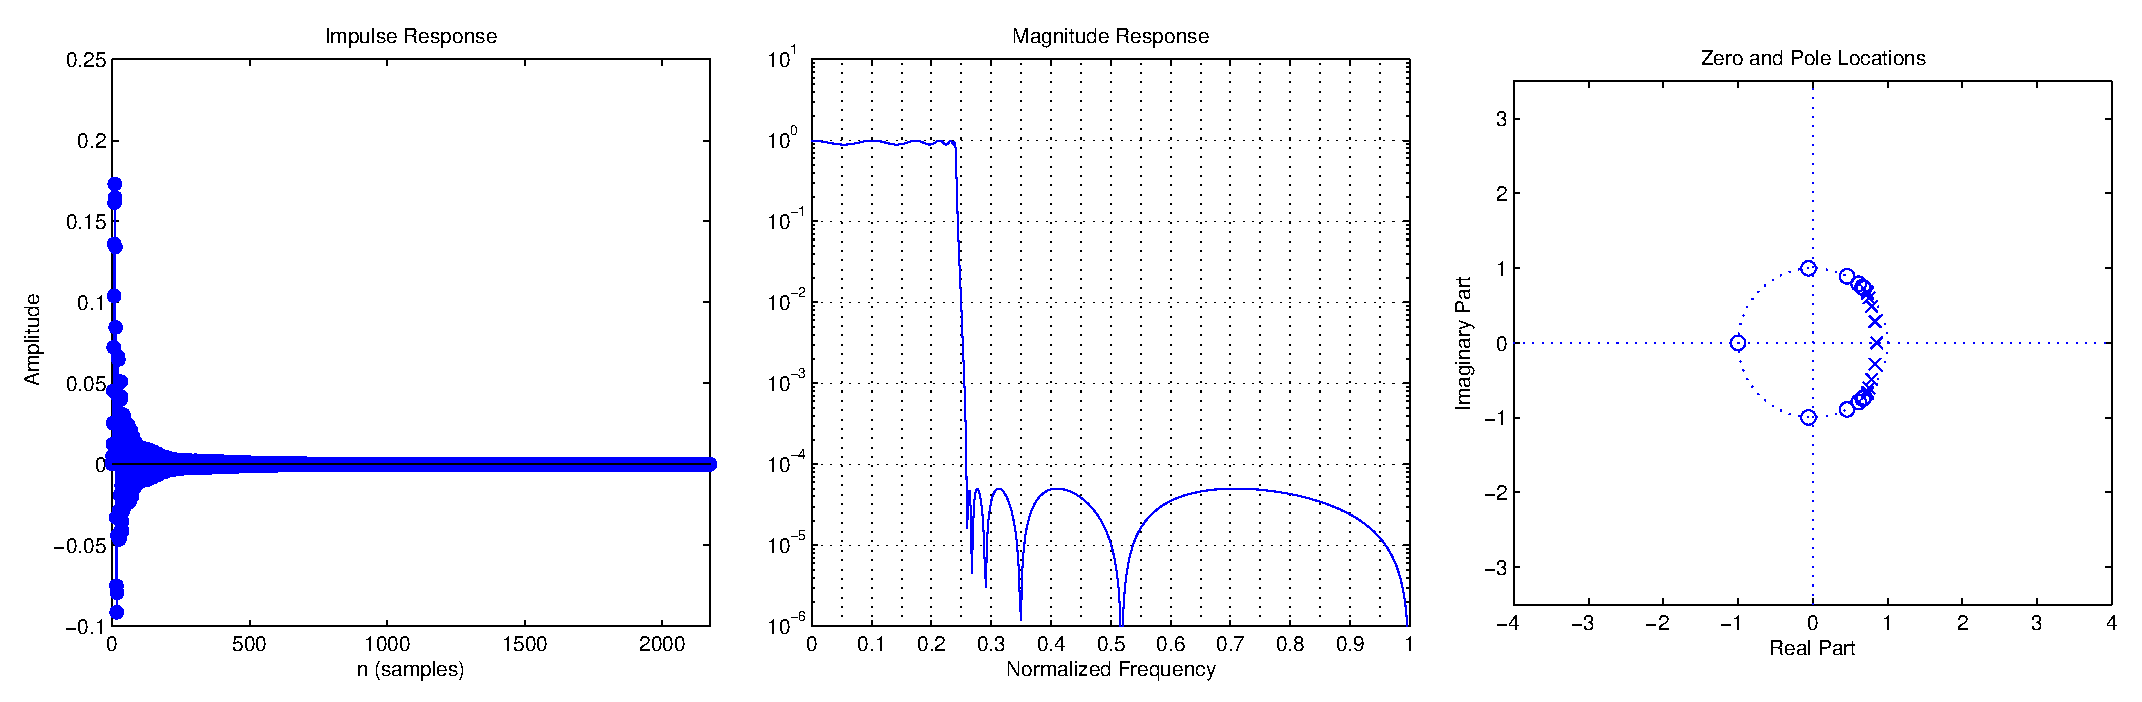
\includegraphics[width=6in]{project7_11.eps}
\caption{Response plots of an IIR lowpass filter}
\label{fig:figure11}
\end{figure}

\newpage
\section*{Exercise 6}
\begin{par}
For Exercise 6, I designed a filter to act on the doorbell.au file from previous weeks' exercises.  The FFT of the audio file is included in Figure 12.  The frequencies of the two chimes are 712Hz and 567Hz.  I opted to use the filter designed by the Parks-McClellan algorithm.  After some trial and error with the exact pass and stop frequencies, I was able to attenuate the higher frequency by 31 dB.
\end{par}

\begin{figure}[htbp]
\centering
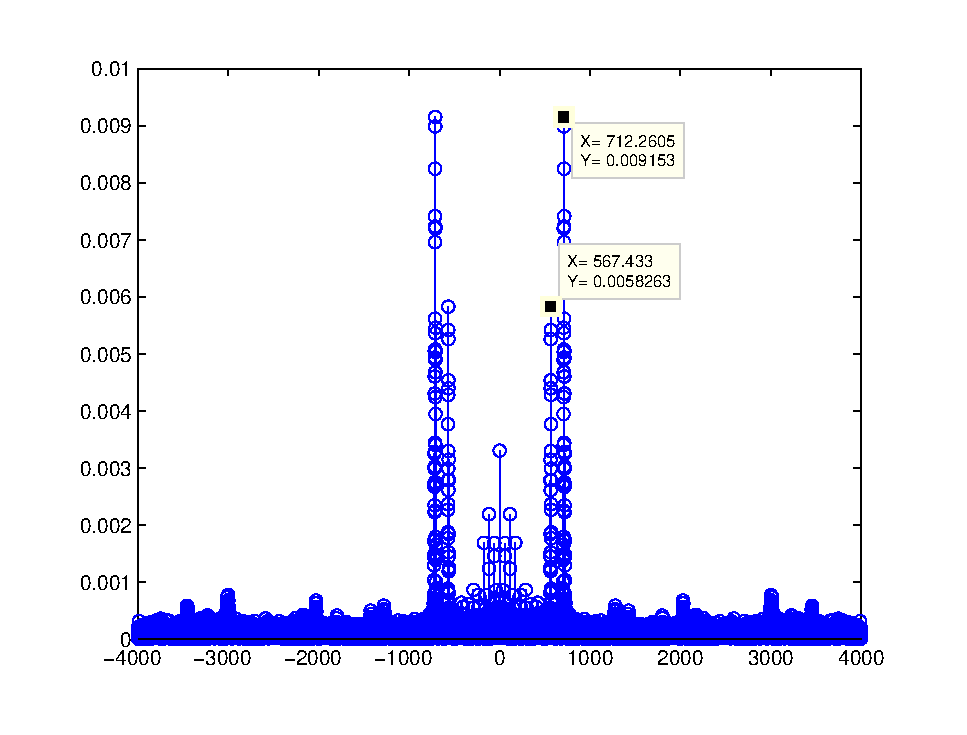
\includegraphics[width=4in]{project6_part3.eps}
\caption{FFT of doorbell.au}
\label{fig:figure12}
\end{figure}

\begin{figure}[htbp]
\centering
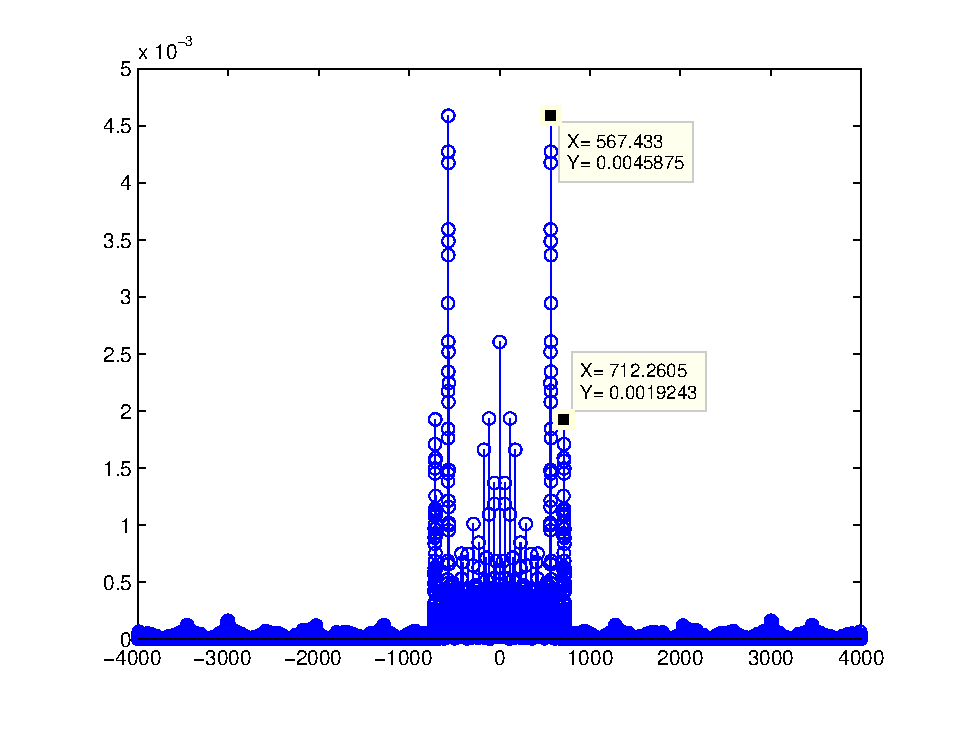
\includegraphics[width=4in]{filterout.eps}
\caption{Output of Filter}
\label{fig:figure13}
\end{figure}

\end{document}

